\section{Results and Analysis}


\subsection{RQ1: Generalisation of FOLTR-ES performance beyond MQ2007/2008}
For answering RQ1 we replicate the results obtained by Kharitonov~\cite{kharitonov2019federated} on the MQ2007 and MQ2008 datasets; we then reproduce the experiment on MSLR-WEB10K and Yahoo datasets, on which FOLTR-ES has not been yet investigated, and we compare the findings across datasets. For these experiments we use antithetic variates, set $B = 4$, use MaxRR as reward signal and for evaluation on clicked items. 

Figure~\ref{label} reports the results obtained by FOLTR-ES on the MQ 2007 dataset\footnote{Similar results were obtained for MQ 2008 and are omitted for space reasons.} with respect to the three click models considered, various settings for the privacy preservation parameter $p$, and the two FOLTR-ES methods (linear and neural). Our results fully replicate those of Kharitonov~\cite{kharitonov2019federated} and indicate the following findings: (1) FOLTR-ES allows for the iterative learning of effective rankers; (2) high values of $p$ (lesser privacy) provide higher effectiveness; 
(3) the neural ranker is more effective than the linear ranker when $p \rightarrow 1$ (small to no privacy), while the linear model is equivalent, or better (for informational clicks) when $p=0.5$. 


However, not all these findings are applicable to the results obtained when considering MSLR-WEB10K and Yahoo, which are displayed in Figures~\ref{label} and~\ref{label}. In particular, we observe that (1) the results for MSLR-WEB10K (and to a lesser extent also for Yahoo) obtained with the informational click model are very unstable, and, regardless of the click model, FOLTR-ES requires more data than with MQ 2007/2008 to arrive at a stable performance, when it does; (2) the neural ranker is less effective than the linear ranker, especially on MSLR-WEB10K. We believe these findings are due to the fact that query-document pairs in MSLR-WEB10K and Yahoo are represented by a larger number of features than in MQ2007/2008. Thus, more data is required for effective training, especially for the neural model; we also note that FOLTR-ES is largely affected by noisy clicks in MSLR-WEB10K. 

%In the previous work, FOLtR-ES is conducted on MQ2007 and MQ2008 datasets~\cite{kharitonov2019federated}. To further study if the algorithm can achieve similar ranking performance on other publicly available LTR datasets. We perform experiments on MSLR-WEB10K dataset using same parameters chosen by~\cite{kharitonov2019federated}, using antithetic variates and setting $B = 4$. 

%Unlike MQ2007 and MQ2008 datasets, FOLtR-ES performed on MSLR-WEB10K shows an opposite finding: the neural ranker dose not consistently perform better that the linear ranker. And for MSLR-WEB10K, FOLtR-ES takes more times on updating the ranker till it achieves the stable performance, which might be caused by larger training queries in MSLR-WEB10K. Figure \ref{fig: mq2007-rq1-1.0}\ref{fig: mslr-rq1-1.0}\ref{fig: mq2007-rq1-0.5}\ref{fig: mslr-rq1-0.5} show the mean batch MaxRR averaged on five data splits in MQ2007 and MSLR-WEB10K with the three click models.

%(Figures lack legend)
%\begin{figure}[H]
%	\centering
%	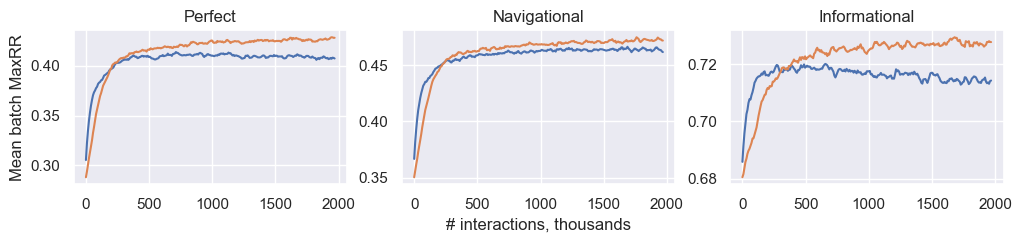
\includegraphics[width=15cm, height=3.5cm]{mq2007_foltr_c2000_p1.0.png}
%	\caption{Mean batch MaxRR for MQ2007 (2000 clients and $p = 0.9$)}
%	\label{fig: mq2007-rq1-1.0}
%\end{figure}
%\begin{figure}[H]
%	\centering
%	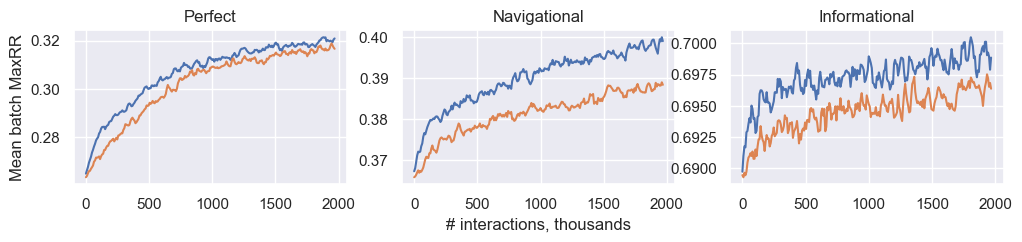
\includegraphics[width=15cm, height=3.5cm]{mslr10k_foltr_c2000_p1.0.png}
%	\caption{Mean batch MaxRR for MSLR-WEB10K (2000 clients and $p = 0.9$)}
%	\label{fig: mslr-rq1-1.0}
%\end{figure}
%
%\begin{figure}[H]
%	\centering
%	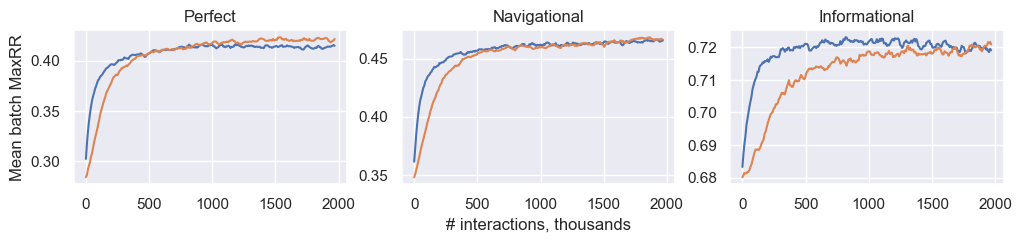
\includegraphics[width=15cm, height=3.5cm]{mq2007_foltr_c2000_p0.5.png}
%	\caption{Mean batch MaxRR for MQ2007 (2000 clients and $p = 0.5$)}
%	\label{fig: mq2007-rq1-0.5}
%\end{figure}
%\begin{figure}[H]
%	\centering
%	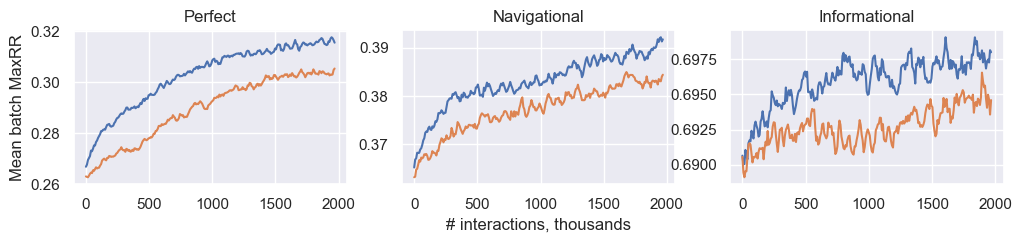
\includegraphics[width=15cm, height=3.5cm]{mslr10k_foltr_c2000_p0.5.png}
%	\caption{Mean batch MaxRR for MSLR-WEB10K (2000 clients and $p = 0.5$)}
%	\label{fig: mslr-rq1-0.5}
%\end{figure}

\subsection{RQ2: Effect of number of clients on FOLTR-ES}
%To answer RQ1, we perform experiments on MSLR-WEB10K dataset with the same FOLtR-ES setup
%Reproducing FOLtR-ES on other datasets

For answering RQ2 we vary thee number of clients involved in FOLTR-ES; we investigate the values \{50, 1,000, 2,000\}. Kharitonov~\cite{kharitonov2019federated} used 2,000 in the original experiments, and the impact of the number . To be able to fairly compare results across number of clients, we fixed the total number of ranker updates to 2,000,000; we also set $B = 4$ and vary the privatization parameter $p$ in \{0.5, 0.9, 1.0\}. We perform these experiments on all three datasets considered in this paper, but we omit to report results for yahoo due to space limitations. 


%To study the influence of number of clients, we perform experiments on MQ2007 and MSLR-WEB10K datasets. We vary the number of clients across \{50, 1000, 2000\} but set the fixed total updating times to 2000000 and set $B = 4$. We also set the privatization parameter $p$ across \{0.5, 0.9, 1.0\}.

Our experiments show that little clients number will reduce the performance in the linear ranker. But for the neural ranker, the difference is minor.

%\begin{figure}[H]
%	\centering
%	\includegraphics[width=16cm, height=8cm]{v0_mq2007_foltr_clients_p09.png}
%	\caption{Mean batch MaxRR for MQ2007 with different client number}
%	\label{fig: mq2007clients}
%\end{figure}
%\begin{figure}[H]
%	\centering
%	\includegraphics[width=15cm, height=3.5cm]{mq2007_foltr_client_linear_p09.png}
%	\caption{Mean batch MaxRR for MQ2007 with different client number (linear ranker and $p = 0.9$)}
%	\label{fig: mq2007-rq2-0.9}
%\end{figure}

\subsection{RQ3: Comparing FOLtR-ES with OLTR baselines}

In order to further study the ranking quality, especially users' experience in FOLtR-ES, we perform experiments on comparing FOLtR-ES with the current state-of-the-art OLTR methods. In this section, we choose Pairwise Differentiable Gradient Descent (PDGD) models as baselines. For a fair comparation, we set up the privacy probability $p = 1$ (lowest privacy) in FOLtR-ES. We perform experiments on MQ2007 and MSLR-WEB10K datasets with simulating 2000 clients.

Based on the experiment results, we can see FOLtR-ES still lags behind OLTR methods in terms of the ranking performance. As the ranking quality is an essential metric for web search engines, future work can be extend to improving ranking performance and in the meantime, protecting users' privacy.

\begin{figure}[H]
	\centering
	\includegraphics[width=16cm, height=8cm]{v0_mq2007_foltr_vs_pdgd_2000clients_p10.png}
	\caption{Mean batch MaxRR for MQ2007 with 2000 clients and $p = 1$}
	\label{fig: mq2007-v0-baseline}
\end{figure}

\begin{figure}[H]
	\centering
	\includegraphics[width=16cm, height=8cm]{v0_mslr_foltr_vs_pdgd_2000clients_p10.png}
	\caption{Mean batch MaxRR for MSLR-WEB10K with 2000 clients and $p = 1$}
	\label{fig: mslr-v0-baseline}
\end{figure}

\begin{figure}[H]
	\centering
	\includegraphics[width=15cm, height=3.5cm]{mq2007_foltr_PDGD_mrr_c2000_p10.png}
	\caption{Mean batch MaxRR for MQ2007 with two FOLtR-ES ranker(2000 clients and $p = 1$) and PDGD baselines}
	\label{fig: mq2007-rq3}
\end{figure}


\subsection{RQ4: Extending FOLtR-ES to other quality metric}


To study the generalisation of FOLtR-ES to other common OLTR evaluation metrics, we use Discounted Cumulative Gain (DCG) to evaluate the users' experience in each interaction. We also compute NDCG@10 with the relevance labels to evaluate the central ranker with test data as we want to explore the stability of  performance in FOLtR-ES.

In terms of nDCG evaluation, although FOLtR-ES achieves decent performance (with nDCG exceed 0.4 except for $Informational$ model), it still falls behind the PDGD baselines.

\begin{figure}[H]
	\centering
	\includegraphics[width=15cm, height=3.5cm]{mq2007_foltr_PDGD_ndcg_c2000_p10.png}
	\caption{Mean batch MaxRR for MQ2007 with(2000 clients and $p = 1$)}
	\label{fig: mq2007-rq4}
\end{figure}


(offline performance (NDCG) for different instantiations of CCM)